\documentclass[a4paper,11pt]{article}
\usepackage{amsmath}
\usepackage{polski}
\usepackage[polish]{babel}
\usepackage[utf8]{inputenc}
\usepackage[T1]{fontenc}
\usepackage{graphicx}
\usepackage{anysize}
\usepackage{enumerate}
\usepackage{times}
\usepackage{plain}
\usepackage{caption}
\usepackage{graphicx}

\begin{document}

\begin{figure}[!htb]
	\centerline{
\includegraphics[scale=1]{agh_logo.jpg}}
\end{figure}

\begin{center}
	\Huge{Wzorce Projektowe\\}
		\vspace{1cm}
		\Large{Implementacja aplikacji wykorzystującej specyfikację HTML5 pozwalającej na przechowywanie informacji w bazie danych przeglądarki oraz synchronizację z bazą centralną.}
	\date{}
%	\maketitle

	\vspace{2cm}
	\Large{	Autorzy:\\
		Konrad Gębczyński\\
		Mateusz Wiater\\
		Rafał Krzyś\\
		Przemysław Michałek\\}

	\newpage

	
\end{center}
\begin{enumerate}
	\item \textbf{{\Large Wprowadzenie}}\\ \\
		\begin{large}
		\hspace*{1cm}
		Poniższa dokumentacja opisuje architekturę oraz styl zaprojektowania systemu dodawania osób fizycznych do bazy danych w postaci aplikacji webowej w standardzie HTML5 \cite{hoy2011html5}.  Technologia HTML5 powstała w 2014 roku i w dobie urządzeń mobilnych jest aktualnie najbardziej wspieranym standardem dla tworzenia stron internetowych, wartymi wspomnienia zaletami HTML5 są:
			\begin{enumerate}
				\item \textbf{Wideo} - HTML5 pozwala na dodanie pliku wideo bezpośrednio na stronę, bez potrzeby używania wtyczki w przeciwieństwie do standardu HTML4, gdzie najczęściej rozwiązywano ten problem dodając powszechnie znanego Flash'a - ta zaleta ma szczególne znaczenie dla użytkowników Apple'a który znany był z konsekwentnego blokowania wtyczki Flash na swoich produktach \cite{johnson2015flash}.
				
				\item \textbf{Geolokacja} - Bardzo ważna cecha w dzisiejszych czasach (chociaż nie zawsze mile widziana), standard HTML5 pozwala serwerowi zlokalizować użytkownika zarówno po adresie IP (dla komputerów stacjonarnych) jak i sygnale GPS, połączeniu Wi-Fi czy Bluetooth \cite{holdener2011html5}.
				
				\item \textbf{Canvas} - Pozwala na lepsze zarządzanie i manipulowanie grafiką bezpośrednio na stronie internetowej. Używa JavaScriptu do dynamicznego rysowania obrazów, jest to tak naprawdę kolejne zastąpienie niemile widzianego Flash'a, więcej o Canvas w artykule \cite{Canvas}.
			\end{enumerate}
		\vspace{1cm}			
		Standard HTML5 został po raz pierwszy zaprezentowany w 2007 roku i otrzymał status rekomendowanego języka w październiku 2014 roku i jest ciągle wspierany jako główna technologia tworzenia stron internetowych, jego najnowsza wersja HTML 5.2 została zatwierdzona w 2017, w planach jest już wersja 5.3, więcej informacji w artykule \cite{html53}.
		
		
		\end{large}


%	\begin{enumerate}
%		\item a^{•}
%		\item b
%		\item c
%		\item d 
%	\end{enumerate}

	\newpage
	\item \textbf{{\Large Cele projektu}}\\ \\
	\begin{large}
	\hspace*{1cm}
			Celem projektu jest stworzenie aplikacji webowej pozwalającej na modyfikowanie bazy danych znajdującej się po stronie serwera z uwzględnieniem sytuacji braku połączenia z siecią: aplikacja powinna odpowiednio dostosować się do sytuacji i w razie braku połączenia dalej zapisywać zmiany w swojej lokalnej bazie danych i w momencie odzyskania połączenia uaktualnić serwerową bazę, podobnie jak jest to rozwiązane w technologii GIT (możliwość wysyłania commit'ów offline i wywoływania komendy \textit{push} w momencie posiadania połączenia z internetem).

	
	\end{large}

	%\newpage
	\item \textbf{{\Large Zasady działania systemu}}\\
	
	\item \textbf{{\Large Opis funkcjonalności}}\\

	\item \textbf{{\Large Schemat procesów}}\\
	
	\item \textbf{{\Large Etapy rozwoju systemu}}\\
	
	\item \textbf{{\Large GUI}}\\
	
		\begin{figure}[!htb]
			\centerline{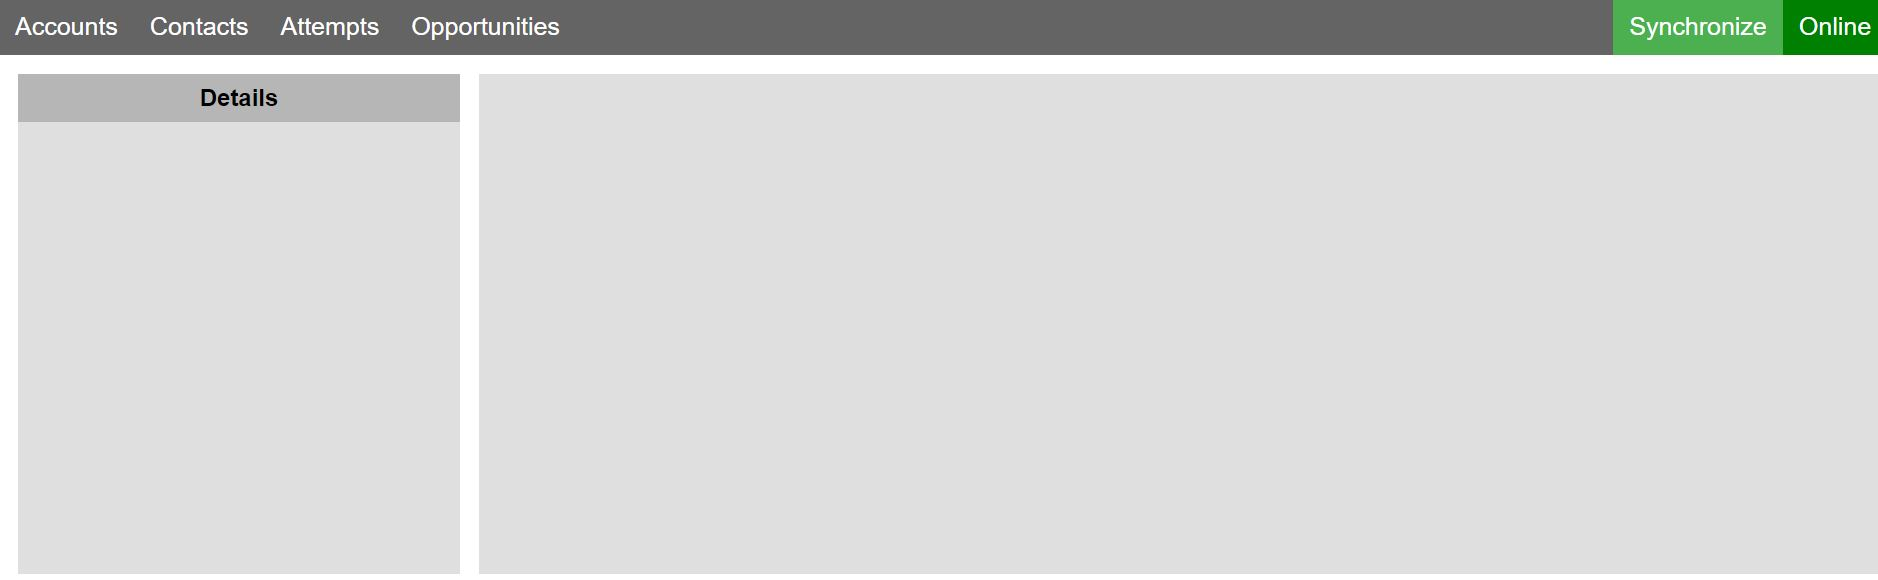
\includegraphics[scale=0.3]{online.jpg}}
		\end{figure}

		\begin{figure}[!htb]
			\centerline{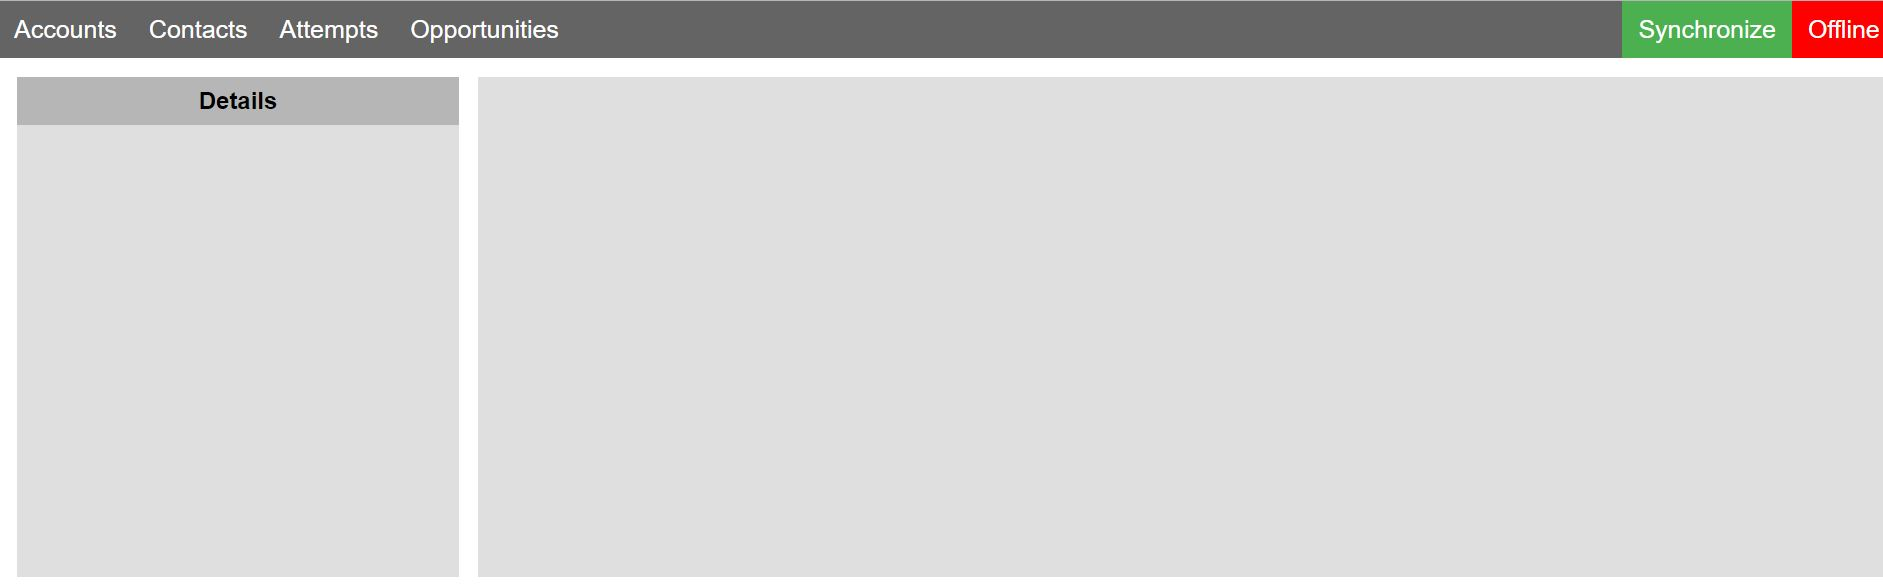
\includegraphics[scale=0.3]{offline.jpg}}
		\end{figure}	
	
	\item \textbf{{\Large Scenariusze / przypadki użycia}}\\
	
	\newpage
	
\bibliographystyle{unsrt}
\bibliography{Bibliografia}
	
\end{enumerate}

\end{document}
